% Task schedule over one hyperperiod — Data Glove Review 2, Figure 4
% Compile: pdflatex sched.tex && pdftoppm -png -r 300 sched.pdf sched
\documentclass[border=8pt]{standalone}
\usepackage{tikz}
\usepackage{pgfplots}
\pgfplotsset{compat=1.18}
\definecolor{pollc}{HTML}{4C7DD9}
\definecolor{inferc}{HTML}{D9534F}
\definecolor{wdc}{HTML}{5B8C5A}
\begin{document}
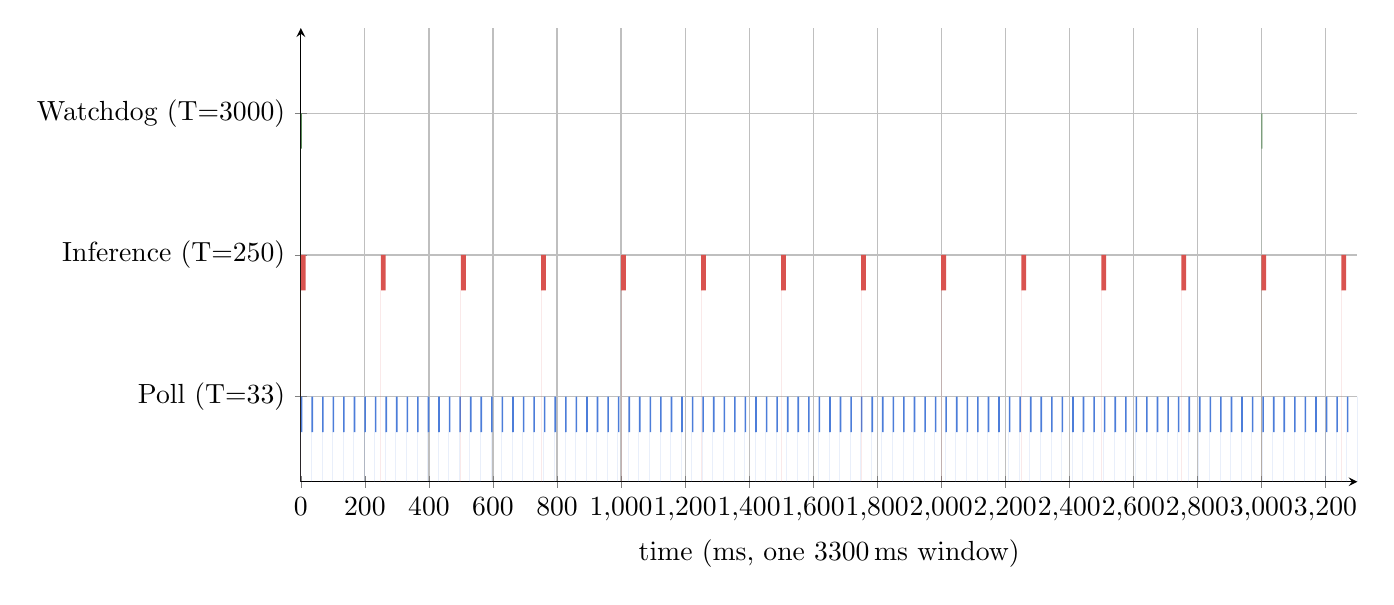
\begin{tikzpicture}
\begin{axis}[
  width=15cm, height=5.2cm,
  xlabel={time (ms, one 3300\,ms window)},
  ytick={1,2,3},
  yticklabels={Poll (T=33), Inference (T=250), Watchdog (T=3000)},
  ymin=0.4, ymax=3.6,
  xmin=0, xmax=3300,
  axis lines=left,
  grid=major,
  minor tick num=0,
  bar width=6pt,
  y=18mm,
  every axis plot/.append style={draw=none}
]
% Poll: every 33ms, ~5ms wide
\foreach \t in {0,33,...,3300} {
  \addplot[fill=pollc,draw=none] coordinates {(\t,1) (\t+5,1) (\t+5,0.75) (\t,0.75)} \closedcycle;
}
% Inference: every 250ms, ~15ms wide
\foreach \t in {0,250,...,3250} {
  \addplot[fill=inferc,draw=none] coordinates {(\t,2) (\t+15,2) (\t+15,1.75) (\t,1.75)} \closedcycle;
}
% Watchdog: once, ~1ms
\addplot[fill=wdc,draw=none] coordinates {(0,3) (3,3) (3,2.75) (0,2.75)} \closedcycle;
\addplot[fill=wdc,draw=none] coordinates {(3000,3) (3003,3) (3003,2.75) (3000,2.75)} \closedcycle;
\node[anchor=west,font=\scriptsize] at (axis cs:3305,1) {5\,ms / 33\,ms frame};
\node[anchor=west,font=\scriptsize] at (axis cs:3305,2) {15\,ms / 250\,ms frame};
\node[anchor=west,font=\scriptsize] at (axis cs:3305,3) {1\,ms / 3000\,ms};
\end{axis}
\end{tikzpicture}
\end{document}
